Dijagrami toka podataka (DFD) prikazuju kako podaci ulaze u sistem, kako ih procesi obrađuju i gde se čuvaju. Najpre je dat dijagram konteksta, koji sistem prikazuje kao jedan proces u interakciji sa spoljnim entitetima, a zatim dijagram prvog nivoa, na kome je sistem razložen na osnovne procese i skladišta podataka.

\subsection{Dijagram konteksta}

Spoljni entiteti sistema su administrator, student i izborna komisija. Administrator unosi podatke o izborima, birački spisak i izborne liste, a od sistema dobija potvrde i poruke o greškama. Student šalje zahtev za glasanje i izabranu listu, a dobija informacije o izborima, potvrdu glasanja i rezultate, odnosno obaveštenje o ponavljanju izbora. Izborna komisija od sistema dobija podatke o izlaznosti i rezultate glasanja, a sistemu šalje potvrdu objavljivanja.

\begin{figure}[H]
    \centering
    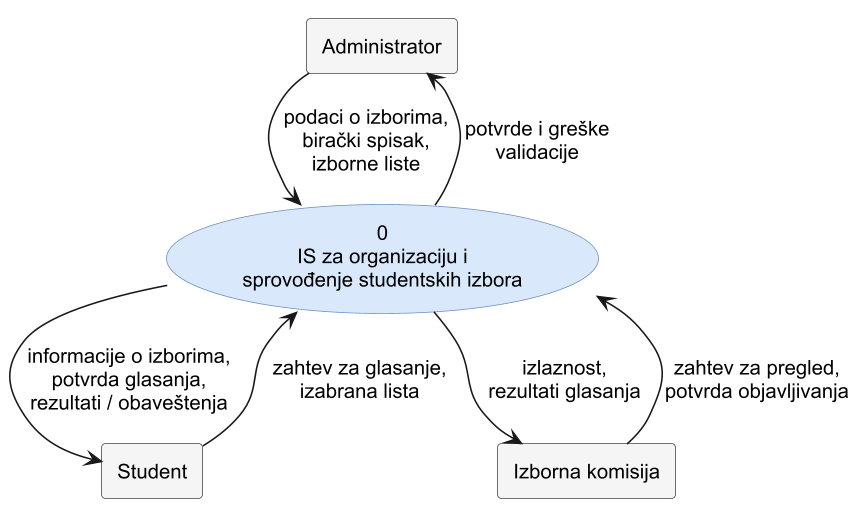
\includegraphics[width=0.85\textwidth]{dfd_kontekst.png}
    \caption{DFD -- dijagram konteksta}
    \label{fig:dfd_kontekst}
\end{figure}

\subsection{Dijagram prvog nivoa}

Na dijagramu prvog nivoa sistem je razložen na šest procesa:
\begin{enumerate}
    \item \textbf{Upravljanje izborima} -- čuva nove izbore sa periodom glasanja u skladištu \textit{D1 Izbori}.
    \item \textbf{Upravljanje biračkim spiskom} -- formira spisak studenata sa pravom glasa u skladištu \textit{D2 Birački spisak}.
    \item \textbf{Upravljanje izbornim listama} -- čuva izborne liste u skladištu \textit{D3 Izborne liste}.
    \item \textbf{Glasanje} -- proverava pravo glasa, upisuje anoniman glas u skladište \textit{D4 Glasovi} i beleži da je student glasao. Glas i identitet studenta se čuvaju u odvojenim skladištima, čime se obezbeđuje tajnost glasanja.
    \item \textbf{Praćenje izlaznosti} -- na osnovu biračkog spiska računa izlaznost i prikazuje je izbornoj komisiji.
    \item \textbf{Obrada i objavljivanje rezultata} -- prebrojava glasove, proverava uslov izlaznosti i, nakon potvrde komisije, objavljuje rezultate ili obaveštenje o ponavljanju izbora.
\end{enumerate}

\begin{figure}[H]
    \centering
    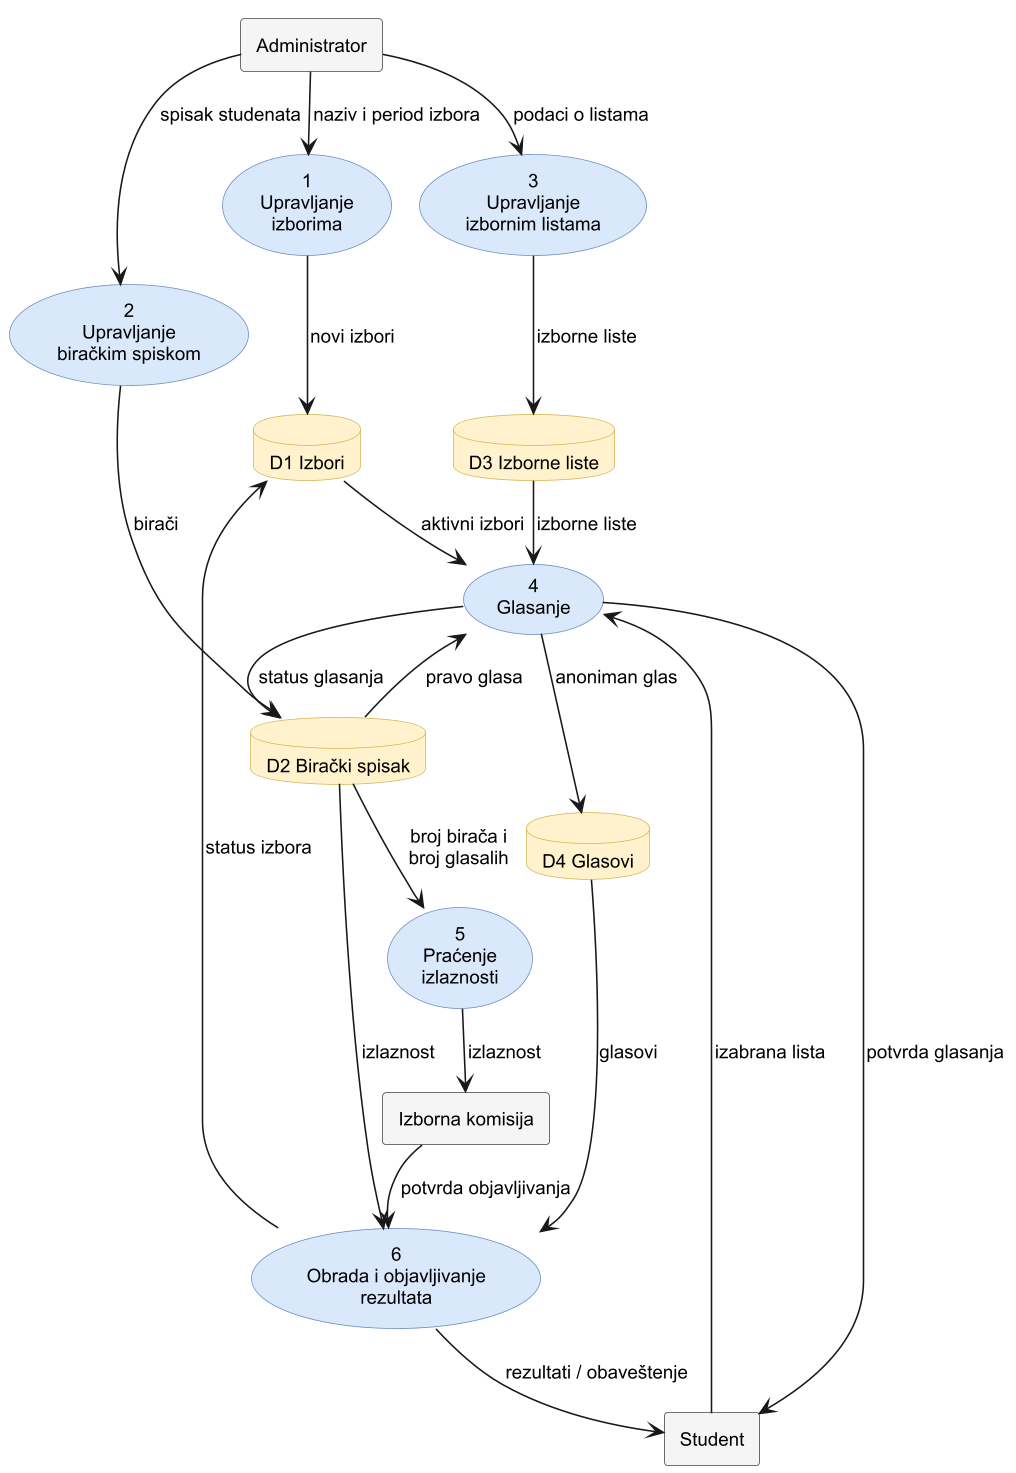
\includegraphics[height=0.72\textheight]{dfd_nivo1.png}
    \caption{DFD -- dijagram prvog nivoa}
    \label{fig:dfd_nivo1}
\end{figure}

\newpage
